% !TeX spellcheck = en_US
\chapter{The choice of corpora for the \context task}\label{chap4}

\section{Introduction}

NLP often relies heavily on the use of language corpora. Employing the terminology of inferential statistics, corpora serve as a \term{sample} from a broader (data) \term{population} that NLP researchers aim to understand. The hope is that patterns identified in the sample will be applicable to the wider population (i.e., a specific kind of language use). However, this assumption is only valid if the sample is \term{representative} of the target population. Otherwise, insights gained from the corpus may not be generalizable to the full spectrum of relevant scenarios. These issues lie at the heart of inferential statistics, yet their applicability to NLP has not been thoroughly explored.

Despite extensive research on the \context problem, the selection of appropriate corpora for this task remains under-discussed. This chapter aims to assess the suitability of various corpora by presenting a case study focused on \context models. These models are tasked with selecting the form of REs in context, or as defined earlier in \chapref{chap3}, RFS.

A central question in this chapter is the impact of corpus selection on \context studies. I hypothesize that the corpora used in prior \context studies are not adequate for the task, and the lessons learned from these studies may not be generally valid. The term \term{previous \context studies} refers specifically to the \grec shared tasks \citep{belz2010generating}.\footnote{This chapter does not cover studies such as \citet{kibrik2016referential} and \citet{castro-ferreira-etal-2016-towards-variation}.} In this context, I examine two corpora used in these shared tasks, \grectwo and \grecp, and argue that they are not suitable for the task at hand.

To determine if the findings from \grec are generally valid (i.e., valid for the intended data population) and to provide a wider perspective, a third corpus, the \wsj portion of OntoNotes \citep{hovy-etal-2006-ontonotes, weischedel2013ontonotes}, is included in the analysis after additional enrichment. To conduct a comprehensive evaluation of the three corpora (\textsc{grec-2.0}, \textsc{grec-people}, and \textsc{wsj}), I replicate the systems from the \grec shared tasks. I use the same ML algorithm and features as the original systems and train the models on all three corpora.\footnote{Methods not considered in \grec, such as E2E neural approaches \citep{ferreira2018neuralreg,cao2019referring,cunha-etal-2020-referring}, are excluded from this discussion as they are not relevant to this specific inquiry.}

This chapter is organized as follows: \sectref{sec:grec} provides an overview of the \grec shared tasks and the corpora involved. \sectref{sec:wsj} offers a detailed examination of the \wsj corpus and its enrichment for this study. \sectref{sec:reconsturction} details study \studA, focusing on a systematic reconstruction and evaluation of various RFS models using the three different corpora. Finally, \sectref{sec:discussionstudya} summarizes the results and findings.

\section{\textsc{Grec} corpora and models}\label{sec:grec}

As described by \citeauthor{belz2010generating}, ``the \grec tasks are about how to generate appropriate references to an entity in the context of a piece of discourse longer than a sentence" \citeyearpar[297]{belz2010generating}. The primary objective of \citeauthor{belz2010generating} was to explore what information influences the selection of REs in context. The \grec shared tasks delve into both content selection (RCS) and form selection (RFS); this chapter, however, concentrates solely on RFS. The RFS task in \grec is defined as a 4-way classification challenge, where systems are required to determine the most suitable choice among a proper name, a description, a pronoun, or an empty RE for referencing entities. In the upcoming sections, I will introduce the specifics of the \grec corpora in \sectref{subsec:greccorpora} and examine the systems that were submitted to these shared tasks in \sectref{subsec:systems}.

\subsection{The corpora used in the \grec shared tasks}\label{subsec:greccorpora}

The \grec studies consist of four shared tasks that use two distinct corpora: \grecmsreight and \grecmsrnine shared tasks employed the \grectwo corpus, while \grecnegnine and \grecnegten used \grecp. Both corpora were derived from the introductory sections of Wikipedia articles. Specifically, the \grectwo corpus comprises 1941 introductory sections across five domains, including people, rivers, mountains, cities, and countries. The \grecp corpus, on the other hand, includes 1000 introductions from articles about composers, chefs, and inventors. In this study, I focus exclusively on articles from the training sets of these corpora, detailed in \tabref{tab:corporachap4}. Examples \REF{ex:berlincity} and \REF{ex:davidchang} illustrate introductory sentences from the \msrcor and \negcor corpora, respectively:


\begin{exe}
	\ex \begin{xlist}
		\ex\label{ex:berlincity} \italunder{Berlin} is the capital city and one of the sixteen federal states of Germany. With a population of 3.4 million in \italunder{its} city limits, \italunder{Berlin} is the country's largest city, and the second most populous city in the European Union. \italunder{Berlin} is an influential center in European politics, culture and science. 
		
		\ex\label{ex:davidchang} \italunder{David Chang} (born 1977) is a noted American chef. \italunder{He} is chef/owner of Momofuku Noodle Bar, Momofuku Ko and Momofuku Ssäm Bar in New York City. \italunder{Chang} attended Trinity College, where \italunder{he} majored in religious studies. In 2003, \italunder{Chang} opened \italunder{his} first restaurant, Momofuku Noodle Bar, in the East Village.
	\end{xlist}
	
\end{exe}


A key distinction between \msrcor and \negcor is their annotation focus. In \msrcor, annotations are limited to references to the main subject of the article, as exemplified in \REF{ex:berlincity} with references to Berlin. In contrast, \negcor annotations encompass all \textit{human} REs. While \REF{ex:davidchang} illustrates annotations pertaining solely to the main character, \negcor contains annotations for every human referent mentioned in each document.

Each RE annotation includes details about its form, grammatical role, and semantic type. While the documents are segmented into paragraphs, finer divisions such as sentences or tokens are not provided. To address this limitation, I used \method{spaCy} for sentence segmentation and tokenization.\footnote{spaCy is a free, open-source Python library for Natural Language Processing (\url{https://spacy.io/}).}

\subsection{The algorithms submitted to the GREC shared tasks}\label{subsec:systems}

The \grec challenges saw submissions of several feature-based algorithms. For the purpose of model reconstruction in this chapter, the feature sets and machine learning (ML) methods of the following submissions were chosen: \citet{hendrickx2008cnts} [\modname{CNTS}], \citet{favre2009icsi}[\modname{ICSI}], \citet{bohnet2008g} [\modname{IS-G}], \citet{jamison2008osu} [\modname{OSU}], and \citet{greenbacker2009udel} [\modname{UDel}]. \tabref{tab:grecsystems} summarizes the names, ML methods, and reported accuracies of these models as documented in \citet{belz2010generating}.

\begin{table}
	\begin{tabularx}{\textwidth}{XlXr}
		\lsptoprule
		Name & Shared Task & ML & Acc \\ \midrule
		\modname{UDel} & \grecmsrnine,\grecnegnine& \method{C5.0} & 77.71 \\
		\modname{ICSI} & \grecmsrnine,\grecnegnine& \method{CRF}& 75.16 \\ 
		\modname{CNTS} & \grecmsreight& \method{MBL}& 72.61 \\ 
		\modname{IS-G} & \grecmsreight& \method{MLP}& 70.78 \\ 
		\modname{OSU} & \grecmsreight& \method{MaxEnt} & 69.82 \\ \lspbottomrule
	\end{tabularx}
	\caption[Original \grec systems.]{\label{tab:grecsystems}
		The first column details the names used for each algorithm in the current study, based on the original names of the systems in \citet{belz2010generating}. The second column indicates the shared task each algorithm was submitted to. The third column (ML) specifies the machine learning algorithm used, and the fourth column (Acc) reports the accuracy of the models on \msrcor as stated in \citet{belz2010generating}.
	}
	
\end{table}

In addition to the variances in the ML algorithms, the feature sets used by each system also significantly differ. The impact of these feature choices on model performance will be thoroughly explored in \chapref{chap5}. 

\section{Enriching \wsj for the \context task}\label{sec:wsj}

\onto, as outlined in \citet{weischedel2013ontonotes}, contains a large collection of texts across seven genres, including broadcast conversation, broadcast news, magazine, newswire, pivot text, telephone conversation, and web data. Unlike the \grec corpora, \onto benefits from comprehensive annotations, including sentence segmentation, tokenization, morpho-syntactic annotation (lemmas, coarse- and fine-grained POS tags), syntactic structure, and shallow semantic details (word sense, coreference). For the purpose of extracting and enriching REs in my study, I use the \term{ONF} files (OntoNotes Normal File), which contain all levels of annotation.

The \wsj dataset, a part of the newswire genre in \onto, was selected for several key reasons. Firstly, the predominance of third-person REs in \wsj makes it ideal for studying RF alternations, which are more pronounced in third-person references compared to the typically pronominal first-person and second-person REs. Secondly, the dataset allows for the addition of paragraph segmentation, a crucial feature for the feature-based studies in Chapters \5 and \6. Lastly, various versions of \wsj have been integral to other REG studies \citep{orita2015discourse,kibrik2016referential,rosiger2018bashi}, making it a valuable and relevant choice for comparison and analysis. In the following sections, I detail the additional annotations made to the \wsj dataset in \sectref{subsec:chap4wsjannotation}, and discuss the specific cases that were excluded from the dataset in \sectref{subsec:chap4wsjexclusion}. 



\subsection{Annotating REs of the \wsj dataset}\label{subsec:chap4wsjannotation}

Enhancing the existing annotations in \wsj, I established a set of rules for automatically annotating REs, subsequently verifying and correcting these annotations manually. Below, I explain the specifics of annotating RF, plurality, animacy/entity type, and gender.

\paragraph*{Referential form} 
While \wsj inherently includes coreferential chain annotations, it lacks specific annotations for RFs. Using POS tag information from the dataset, REs were automatically labeled as \val{pronoun}, \val{description}, or \val{name}.\footnote{Here, the term \term{name} is used synonymously with \term{proper name}.} Despite the high accuracy of this method, relying solely on POS tags can occasionally result in misannotations. For instance, the phrase \intext{the United States} might be mistakenly labeled as a description based on its initial determiner, despite being a proper name. To correct such inaccuracies, I conducted a manual review of these tags.\footnote{These tags are further categorized into more detailed classifications, taking into account factors such as expression length and modification, as discussed in \citep{belz2007generation}. However, this book does not delve into these finer distinctions.} \REF{ex:reform} from document \example{wsj-0990} illustrates various REs with their corresponding annotations.

\begin{exe}
	\ex\label{ex:reform}
	\italunder{Their}$_{\texttt{pronoun}}$ tone was good-natured, with \italunder{Mr. Packwood}$_{\texttt{name}}$ saying\\ \italunder{he}$_{\texttt{pronoun}}$ intended to offer \italunder{the proposal}$_{\texttt{description}}$ again and again on future legislation and \italunder{Sen. Mitchell}$_{\texttt{name}}$ saying \italunder{he}$_{\texttt{pronoun}}$ intended to use procedural means to block \italunder{it}$_{\texttt{pronoun}}$ again and again.
\end{exe}

\paragraph*{Plurality} The \term{plurality} feature in the annotation process identifies whether a referent is \val{plural} or \val{singular}. This classification is based on the content of the REs. When a coreferential chain contained a singular pronominal form, such as \intext{he} or \intext{she}, the entire chain was tagged as \val{singular}. In contrast, if the chain included a plural pronoun, then \val{plural} was assigned to all its members. Cases that lacked explicit pronominal forms within the coreferential chains were annotated manually.

\paragraph*{Animacy/entity type} 

For the animacy or entity type annotation, the name entity annotations already present in the corpus, as documented in \citep[21]{weischedel2012ontonotes}, were initially used. These annotations were then reviewed and confirmed manually. The category of animacy/entity type includes a variety of values, such as \val{person}, \val{organization}, \val{location}, among others.

\paragraph*{Gender} The feature \term{gender} indicates the gender of individual human referents. Referential chains with at least one male pronominal form were assigned the tag \val{male}, and those with female pronominal forms were given the tag \val{female}. I tagged all other cases as \val{other}. I checked and manually corrected the annotations if necessary.


\subsection{REs excluded from the \wsj dataset}\label{subsec:chap4wsjexclusion}

This section outlines the criteria used to exclude certain REs from the \wsj dataset.

\paragraph*{First-person and second-person REs} 
Given the minimal RF alternation in first-person and second-person REs, these have been excluded from the dataset. The exclusion process involved first converting the REs to lowercase and then omitting the following pronominal forms, amounting to 1847 REs in total:

\begin{quote}
	First-person and second-person REs= \val{\{"i", "my", "mine", "me", "you", "your", "yours", "we", "us", "ours", "our"\}}.
\end{quote}

In addition to first-person and second-person REs, certain REs were also excluded from the set of 42,032 third-person REs. The criteria for their exclusion include:

\paragraph*{Appositives} 
The \onto corpus annotates two distinct types of referential relations, namely \term{IDENT} and \term{APPOS}, as described in \citep{weischedel2012ontonotes}:

\begin{itemize}
	\item IDENT: Identity relation includes the annotation of REs with anaphoric mentions (coreference).
	\item APPOS: Apposition relation contains the annotation of the head of an appositive phrase along with one or more attributes associated with the head.
\end{itemize}

\figref{fig:chains} provides an example of both identity and appositive chains. In the upper portion of the figure, an IDENT chain is depicted where the REs \intext{Gary Hoffman, a Washington lawyer specializing in intellectual-property cases}, \intext{he}, and \intext{He} are in a coreferential relationship. Conversely, the lower part showcases an appositive chain where \intext{Gary Hoffman} is the head, and \intext{a Washington lawyer specializing in intellectual-property cases} functions as the attribute, providing additional information about the head. For the purposes of this study, appositive chains were excluded from the dataset.

{\refstepcounter{figure}
	\tcbset{
		colback=white,
		boxrule=0.1pt,
		colframe=black!75,
		fonttitle=\bfseries}
	\begin{tcolorbox}[text width=11cm]
		\textsc{\textbf{ident chain}}\\
		\textsc{\textbf{re 1:}} Gary Hoffman, a Washington lawyer specializing in intellectual - property cases, \\
		\textsc{\textbf{re 2:}} he\\
		\textsc{\textbf{re 3:}} He
		\tcblower
		\textsc{\textbf{appos chain}}\\
		\textsc{\textbf{head:}} Gary Hoffman\\
		\textsc{\textbf{attrib:}}	a Washington lawyer specializing in intellectual - property cases
	\end{tcolorbox}
	\label{fig:chains}
	\begin{center}
		Figure \thefigure: An example of IDENT and APPOS chains in the \wsj corpus.
	\end{center}
}

\paragraph*{Non-coreferential chains}

Consider the scenario illustrated in \REF{ex:non-referring}, where \intext{a criminal defendant} and \intext{a criminal defendant who chooses not to testify} are treated as separate but nested REs with a coreferential relationship. In such instances, only the maximal span, namely \intext{a criminal defendant who chooses not to testify}, is considered as an RE, while the shorter expression \intext{a criminal defendant} is excluded from the analysis.



\begin{exe}
	\ex\label{ex:non-referring} This privilege against self-incrimination precludes the drawing of an adverse inference against \italunder{[[a criminal defendant] who chooses not to testify]}.
\end{exe}

\paragraph*{Verbal and coordinated expressions}

In addition to excluding appositives and non-coreferential instances, I also omitted other specific cases from the analysis. These include verbal expressions and coordinated expressions where the NPs do not align in terms of their \texttt{person} attribute. For instance, in \REF{ex:verbal}, the verbal expression \intext{applied} is coreferential with the noun phrase \intext{its application}. However, due to its verbal nature, \intext{applied} is not included in the dataset. Similarly, in \REF{ex:coordinated}, there is a coordination between \intext{Mr. Apple}, a third-person REs, and \intext{I}, a first-person RE. The difference in \texttt{person} information between these coordinated NPs led to their exclusion from the analysis.

\begin{exe}
	\ex\label{ex:verbal} An official of the Palestinian Olympic Committee said the committee first \italunder{applied} for membership in 1979 and renewed its application in August of this year.
\end{exe} 

\begin{exe}
	\ex\label{ex:coordinated} All of which has enabled those of us in Washington who enjoy wallowing
	in such things to go into high public dudgeon, as \italunder{Mr. Apple and I} did the other night on ABC’s ``Nightline."
\end{exe} 

With these exclusions applied, the dataset retains 30,471 REs. The following summary provides a comprehensive overview of the \wsj dataset alongside the other two corpora discussed earlier. 
 
\section{Interim summary}

Sections \sectref{sec:grec} and \sectref{sec:wsj} have introduced the three corpora -- $\wsj$, \msrcor, and $\negcor$ -- that will be pivotal in study \studA. \tabref{tab:corporachap4} offers an in-depth comparison of these corpora, encompassing various characteristics and referential expression distributions.

\begin{table}
	\begin{tabularx}{\textwidth}{Xrrr}
		\lsptoprule
		Characteristics & \msrcor & \negcor & \wsj \\
		\midrule
		Genre & Wikipedia & Wikipedia & Newspaper\\
		Number of documents& 1655 & 808 & 585 \\ 
		Word/doc (mean) & 148.3 & 129.3 & 530.7 \\ 
		Sentence/doc (mean)& 7.2 & 5.8 & 25 \\ 
		Paragraph/doc (mean)& 2.3 & 2.2 & 11 \\ 
		Referent/doc (mean) & 1 & 2.6 & 15 \\ 
		RE/doc (mean) & 7.1 & 10.9 & 52.1 \\ 
		Total number of REs & 11,705 & 8378 & 30,471 \\ 
		\texttt{Description} n(\%) & 1620(13.84\%) & 335(4\%) & 12,020(39.45\%) \\ 
		\texttt{Name} n(\%) & 4459(38.09\%) & 3417(40.79\%) & 11,164(36.64\%) \\ 
		\texttt{Pronoun} n(\%) & 4891(41.79\%) & 4084(48.75\%) & 7287(23.91\%) \\ 
		\texttt{Empty} n(\%) & 735(6.28\%) & 542(6.47\%) & - \\
		\lspbottomrule
	\end{tabularx}
	\caption[A detailed overview of \msrcor, \negcor, and \wsj corpora.]{\label{tab:corporachap4} A comparison of \msrcor, \negcor, and \wsj in terms of their length-related features and RF distributions.
	}
\end{table}

As the table shows, there are considerable differences in length-related features and RE distribution between \msrcor and \negcor, on the one hand, and \wsj, on the other. For instance, while the occurrence of (proper) names is relatively consistent across all corpora, descriptions show a marked variance, being most frequent in \wsj (39.45\% of its total REs) compared to their presence in \msrcor (\sim14\%) and \negcor (\sim4\%). The next section will delve into the methodology and implications of reconstructing the \grec systems with these diverse corpora, aiming to provide insights into how these differences influence the outcomes and interpretations in the study.

\section{Study A: Reconstruction of the \grec RFS models}\label{sec:reconsturction}

Study \studA is dedicated to the meticulous reconstruction of several RFS models.\footnote{Refer to \citet{same-etal-2023-models} for an updated version of study \studA, which also integrates pretrained Language Models.} The primary objective of this study is to assess whether the original corpora employed in these models were adequately suited for their intended tasks. This examination is crucial for understanding the effectiveness and generalizability of the findings derived from these models. The section unfolds as follows: \sectref{subsec:inspection} delves into the necessity of thoroughly inspecting the corpora used in \context studies. It aims to evaluate their representativeness and appropriateness in capturing the nuances of the RFS task. \sectref{subsec:refcategories} describes the various RF categories employed in RFS studies. \sectref{algoreconstruction} explains the methodology behind the reconstruction of the RFS models, detailing the steps taken to replicate the original models using the selected corpora. Lastly, \sectref{sec:algoevaluation} presents a comprehensive evaluation of the reconstructed models.

\subsection{The need for a closer inspection of \context corpora}\label{subsec:inspection}

As previously discussed, the \grec tasks have introduced several feature-based \context models into the realm of REG \citep{bohnet2008g,greenbacker2009udel,orasan-dornescu-2009-wlv}. However, certain aspects of the \grec corpora raise concerns about their suitability for these tasks. This section elaborates on these issues and explains the rationale for incorporating a third corpus in this study.

\paragraph*{Representativity} 
Despite the notable differences in annotation practices between the \msrcor and \negcor corpora, both draw from the same genre of text, namely, Wikipedia articles. Given that one of the principal objectives of this chapter is to assess the representativeness of these resources, I have incorporated a third corpus into the study. This additional corpus contrasts with \msrcor and \negcor not only in genre but also in terms of length and various other features. The inclusion of this divergent corpus will allow for a more comprehensive analysis, shedding light on how genre and other textual characteristics impact the outcome of the models.

\paragraph*{The \grec task definition}

According to the \grec task definition cited in \sectref{sec:grec}, the minimum requirement is to generate REs in a piece of text longer than \emph{a sentence}. Upon evaluating the two corpora, it was observed that 80 documents in \msrcor, representing 4.8\% of the training set, and 114 documents in \negcor, accounting for 14.1\% of the training set, comprise only a single sentence. Consequently, these documents fail to meet the minimum task requirement. In contrast, such instances are notably rare in the \wsj corpus, occurring in merely two documents (0.3\%). This disparity underscores the significance of conducting an initial evaluation of corpora to confirm their alignment with the primary requirements of the study's targeted task.

\paragraph*{The distribution of RFs} 
As illustrated in \tabref{tab:corporachap4}, the two predominant RF types in the \grec corpora, specifically pronouns and proper names, collectively constitute a significant portion of the referential instances: 80\% in \msrcor and 89.5\% in \negcor. The remaining referential forms, which include descriptions and empty references, contribute to approximately 20\% of the instances in \msrcor and around 10\% in \negcor. This distribution presents a crucial question for the study: Does this imbalance in the frequency of different RF types impact the effectiveness of the RFS algorithms? More specifically, the study seeks to investigate whether RFs that appear less frequently are accurately predicted by these algorithms.

Incorporating the \wsj corpus, with its distinct distribution of RF types, provides an opportunity to explore these questions in a varied context. The diverse distribution of RFs in \wsj may offer insights into how algorithms perform across a more balanced range of referential forms. 

\subsection{RF categories considered}\label{subsec:refcategories}
\context studies have explored various RF classifications. These include:

\begin{itemize}
	\item 2-Way (binary) classification \citep{mccoy1999generating,henschel2000pronominalization,poesio2004centering}: This classification distinguishes between pronominal and non-pronominal REs.
	\item 3-Way classification \citep{kibrik2016referential}: Here, REs are categorized as either a pronoun, a description, or a proper name.
	\item 4-Way classification \citep{belz2010generating}: This approach includes an additional category of empty forms, along with pronouns, descriptions, and proper names.
	\item 5-Way classification \citep{castro-ferreira-etal-2016-towards-variation}: This classification adds demonstrative forms to the four categories mentioned above.
\end{itemize}


In the context of this study, a faithful reconstruction would ideally adhere to the 4-way classification model employed in the \grec tasks. However, a notable limitation is the absence of annotations for empty references in the \wsj corpus. To accommodate this, I modify the approach to focus on a 3-way classification task, considering the labels \val{pronoun}, \val{description}, and \val{(proper) name}. This adaptation, though necessary due to the dataset constraints, might impact the study's outcomes, as it may affect the generalizability and comparability of the findings with those from the original \grec tasks.

\subsection{Architecture of the models}\label{algoreconstruction}
In assessing the performance of the algorithms across different corpora, two approaches were considered:

\begin{itemize}
	\item Construction of \negcor and \wsj algorithms: This method involves constructing the algorithms for these two corpora and comparing their accuracy with the reported accuracy of the \msrcor algorithms in \citet{belz2010generating}, as shown in \tabref{tab:grecsystems}.
	
	\item Reconstruction of algorithms for all three corpora: This approach entails reconstructing the algorithms for \msrcor, \negcor, and \wsj using the feature sets and ML methods detailed in \citet{belz2010generating}.
	
\end{itemize}

I have opted for the second solution based on two key considerations. Firstly, there is a lack of clarity regarding the specific parameters employed in the algorithms submitted to \grec.\footnote{I contacted the developers of the models submitted to the \grec shared tasks to obtain information about their models' parameters, but unfortunately, the responses received did not provide conclusive details.} Given this uncertainty, constructing algorithms for the \wsj and \negcor corpora using new parameters and then comparing their performance to the original \msrcor algorithms' accuracy might yield inaccurate or misleading results. 

Secondly, a comprehensive evaluation of the algorithms' effectiveness in predicting \textit{each} class necessitates a per-class analysis of the predictions. Such a detailed level of evaluation is not provided in the \grec report \citep{belz2010generating}.

As indicated in \sectref{sec:grec}, this study involves the reconstruction of five systems originally submitted to the \grec tasks. These systems are based on five distinct ML algorithms, each implemented using specific software packages and configurations:

\begin{enumerate}
	\item Conditional Random Field [CRF]: The \method{crfsuite} package (\url{https://cran.r-project.org/web/packages/crfsuite/}) is used for training CRF models. Settings include 3000 iterations and Stochastic Gradient Descent (SGD) with L2-regularization (\val{l2sgd}) as the learning method.
	\item C5.0 Decision Tree [C5.0]: The \method{C5.0} R package \citep{kuhn2018package} is employed to construct decision trees. The number of boosting iterations (trials) is set to 3, using information gain (entropy) as the splitting criterion.
	\item Memory-Based Learning [KNN]: While \citet{hendrickx2008cnts} referenced the TiMBL package \citep{daelemans2007timbl} for Memory-Based Learning, I implement the k-Nearest Neighbors (KNN) algorithm, a direct descendant of Memory-Based Learning \citep{daelemans2007timbl}. The \method{caret} package, with the method \method{knn}, is used for this implementation.
	\item Maximum Entropy Classifier [MaxEnt]: The \method{multinom} algorithm from the \method{nnet} R
	package is used, given the theoretical similarity of the Maximum Entropy classifier to multinomial logistic regression. This choice was made as the original \method{maxent} package has since been deprecated.
	\item Multilayer Perceptron [MLP]: The MLP is implemented using the \method{Keras} package. The model includes two hidden layers with 16 and 8 units respectively, employing the rectified linear activation function (ReLU) for the hidden layers and the Sigmoid activation function for the output layer. The model is trained over 50 epochs, with a batch size of 50 samples.
\end{enumerate}



I have developed feature sets for each of the three corpora -- \msrcor, \negcor, and $\wsj$ -- on which the respective algorithms are trained. \figref{fig:algoscheme} illustrates the reconstruction process for each algorithm. As an example, the first dashed box in the figure indicates that the \modname{UDel} feature set, coupled with its ML method C5.0, is employed to train decision trees for all three corpora.\footnote{A comprehensive description of the features used in these systems is detailed in \chapref{chap5}.} Applying these feature sets and ML methods across the three corpora results in a total of 15 distinct classifiers. For the purpose of training and evaluating these models, the data in each corpus is partitioned into two segments: 70\% is allocated for the training and development sets, and the remaining 30\% forms the test set. 



\tikzset{every picture/.style={line width=0.75pt}} %set default line width to 0.75pt        
\begin{figure}[htbp]
    \centering
    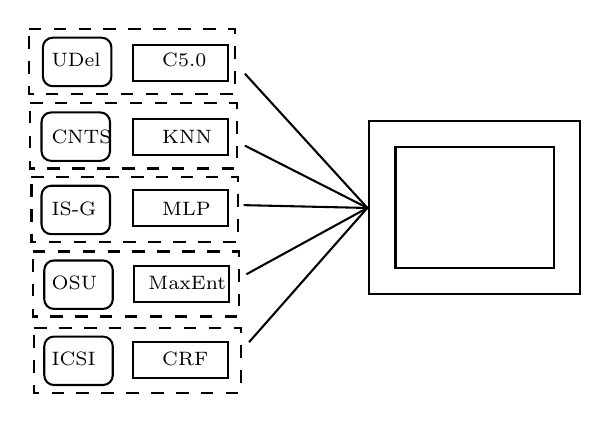
\begin{tikzpicture}[x=0.50pt,y=0.50pt,yscale=-1,xscale=1]
%uncomment if require: \path (0,300); %set diagram left start at 0, and has height of 300

%Rounded Rect [id:dp11696032525693911] 
\draw   (6,30) .. controls (6,26.13) and (9.13,23) .. (13,23) -- (48.5,23) .. controls (52.37,23) and (55.5,26.13) .. (55.5,30) -- (55.5,51) .. controls (55.5,54.87) and (52.37,58) .. (48.5,58) -- (13,58) .. controls (9.13,58) and (6,54.87) .. (6,51) -- cycle ;
%Rounded Rect [id:dp07799259931950897] 
\draw   (5,84) .. controls (5,80.13) and (8.13,77) .. (12,77) -- (47.5,77) .. controls (51.37,77) and (54.5,80.13) .. (54.5,84) -- (54.5,105) .. controls (54.5,108.87) and (51.37,112) .. (47.5,112) -- (12,112) .. controls (8.13,112) and (5,108.87) .. (5,105) -- cycle ;
%Rounded Rect [id:dp6057157286378516] 
\draw   (5,137) .. controls (5,133.13) and (8.13,130) .. (12,130) -- (47.5,130) .. controls (51.37,130) and (54.5,133.13) .. (54.5,137) -- (54.5,158) .. controls (54.5,161.87) and (51.37,165) .. (47.5,165) -- (12,165) .. controls (8.13,165) and (5,161.87) .. (5,158) -- cycle ;
%Rounded Rect [id:dp05149661187443377] 
\draw   (7,191) .. controls (7,187.13) and (10.13,184) .. (14,184) -- (49.5,184) .. controls (53.37,184) and (56.5,187.13) .. (56.5,191) -- (56.5,212) .. controls (56.5,215.87) and (53.37,219) .. (49.5,219) -- (14,219) .. controls (10.13,219) and (7,215.87) .. (7,212) -- cycle ;
%Rounded Rect [id:dp5106057202150704] 
\draw   (7,246) .. controls (7,242.13) and (10.13,239) .. (14,239) -- (49.5,239) .. controls (53.37,239) and (56.5,242.13) .. (56.5,246) -- (56.5,267) .. controls (56.5,270.87) and (53.37,274) .. (49.5,274) -- (14,274) .. controls (10.13,274) and (7,270.87) .. (7,267) -- cycle ;
%Shape: Rectangle [id:dp4932792416812033] 
\draw   (71,28) -- (139.5,28) -- (139.5,54) -- (71,54) -- cycle ;
%Shape: Rectangle [id:dp18275608668220578] 
\draw   (71,82) -- (139.5,82) -- (139.5,108) -- (71,108) -- cycle ;
%Shape: Rectangle [id:dp49550112521417855] 
\draw   (71,133) -- (139.5,133) -- (139.5,159) -- (71,159) -- cycle ;
%Shape: Rectangle [id:dp7299903908595833] 
\draw   (72,188) -- (140.5,188) -- (140.5,214) -- (72,214) -- cycle ;
%Shape: Rectangle [id:dp29994453006627353] 
\draw   (71,243) -- (139.5,243) -- (139.5,269) -- (71,269) -- cycle ;
%Shape: Frame [id:dp0788278471216437] 
\draw   (242,83) -- (394,83) -- (394,208.5) -- (242,208.5) -- cycle(375.18,101.83) -- (260.83,101.83) -- (260.83,189.68) -- (375.18,189.68) -- cycle ;
%Straight Lines [id:da17320760077273079] 
\draw    (152,49) -- (240.5,146) ;
%Straight Lines [id:da17575985418730822] 
\draw    (152,101) -- (240.5,146) ;
%Straight Lines [id:da30612580255952593] 
\draw    (151,144) -- (238.5,146) ;
%Straight Lines [id:da8325128920363636] 
\draw    (153,194) -- (240.5,146) ;
%Straight Lines [id:da9535817232752342] 
\draw    (155,243) -- (240.5,146) ;
%Shape: Rectangle [id:dp03213107417825167] 
\draw  [dash pattern={on 4.5pt off 4.5pt}] (-4.25,16.5) -- (145,16.5) -- (145,63.5) -- (-4.25,63.5) -- cycle ;
%Shape: Rectangle [id:dp5683744790831955] 
\draw  [dash pattern={on 4.5pt off 4.5pt}] (-3.25,70.5) -- (146,70.5) -- (146,117.5) -- (-3.25,117.5) -- cycle ;
%Shape: Rectangle [id:dp09403085065069972] 
\draw  [dash pattern={on 4.5pt off 4.5pt}] (-2.25,123.5) -- (147,123.5) -- (147,170.5) -- (-2.25,170.5) -- cycle ;
%Shape: Rectangle [id:dp8830923797784842] 
\draw  [dash pattern={on 4.5pt off 4.5pt}] (-1.25,177.5) -- (148,177.5) -- (148,224.5) -- (-1.25,224.5) -- cycle ;
%Shape: Rectangle [id:dp5129842925423971] 
\draw  [dash pattern={on 4.5pt off 4.5pt}] (-0.25,232.5) -- (149,232.5) -- (149,279.5) -- (-0.25,279.5) -- cycle ;

% Text Node
\draw (10,32) node [anchor=north west][inner sep=0.75pt]   [align=left] {{\scriptsize \modname{UDel}}};
% Text Node
\draw (10,88) node [anchor=north west][inner sep=0.75pt]  [font=\scriptsize] [align=left] {\modname{CNTS}};
% Text Node
\draw (10,140) node [anchor=north west][inner sep=0.75pt]  [font=\scriptsize] [align=left] {\modname{IS-G}};
% Text Node
\draw (10,193) node [anchor=north west][inner sep=0.75pt]  [font=\scriptsize] [align=left] {\modname{OSU}};
% Text Node
\draw (10,248) node [anchor=north west][inner sep=0.75pt]  [font=\scriptsize] [align=left] {\modname{ICSI}};
% Text Node
\draw (90,32) node [anchor=north west][inner sep=0.75pt]  [font=\scriptsize] [align=left] {\method{C5.0}};
% Text Node
\draw (90,88) node [anchor=north west][inner sep=0.75pt]  [font=\scriptsize] [align=left] {\method{KNN}};
% Text Node
\draw (90,140) node [anchor=north west][inner sep=0.75pt]  [font=\scriptsize] [align=left] {\method{MLP}};
% Text Node
\draw (80,193) node [anchor=north west][inner sep=0.75pt]  [font=\scriptsize] [align=left] {\method{MaxEnt}};
% Text Node
\draw (90,248) node [anchor=north west][inner sep=0.75pt]  [font=\scriptsize] [align=left] {\method{CRF}};
% Text Node
\draw (280,111) node [anchor=north west][inner sep=0.75pt]  [font=\scriptsize] [align=left] {\msrcor};
% Text Node
\draw (280,140) node [anchor=north west][inner sep=0.75pt]  [font=\scriptsize] [align=left] {\negcor};
% Text Node
\draw (280,168) node [anchor=north west][inner sep=0.75pt]  [font=\scriptsize] [align=left] {\wsj};


\end{tikzpicture} 

    
    \caption[Feature sets and ML methods.]{The feature sets and the ML methods of the five GREC algorithms used to train classifiers on the three corpora.} 
    \label{fig:algoscheme}
\end{figure}


\subsection{Evaluation of the algorithms}\label{sec:algoevaluation}

This section is dedicated to a thorough evaluation of the reconstructed algorithms. The primary focus is on assessing the accuracy of the models, consistent with the metrics used in the \textsc{grec-msr} shared tasks. As documented in \tabref{tab:grecsystems}, accuracy was the sole measure reported for all of these systems, while precision and recall were detailed only in the context of the \textsc{grec-neg} shared tasks (refer to \citealt{belz2010generating} for more on this decision). Thus, the evaluation in \sectref{subsec:overallacc} will primarily report on the accuracy of each model across the three corpora.

Following the accuracy assessment, a Bayes Factor (BF) analysis is conducted in \sectref{subsec:bayes}. This analysis will provide statistical evidence to determine whether the observed accuracy rates across different models and corpora stem from similar or different distributions.

Finally, a per-class evaluation of the predictions is carried out in \sectref{perclasseval}, which aims to dissect the performance of the algorithms for each referential form class (e.g., pronoun, description, proper name). This step is essential to evaluate the true effectiveness of the algorithms, as it reveals how well they perform for each specific category of RF.


\subsubsection{Accuracy of the models}\label{subsec:overallacc}
\tabref{tab:systems} presents the overall accuracy achieved by each model in the 3-way classification task.

\begin{table}
\begin{tabularx}{.8\textwidth}{Xrrrrr}
\lsptoprule
& \modname{UDel} & \modname{CNTS} & \modname{IS-G} & \modname{ICSI} & \modname{OSU} \\
\midrule
\msrcor & 0.67 & 0.68 & 0.69 & 0.72 & 0.70 \\
\negcor & 0.80 & 0.75 & 0.78 & 0.78 & 0.79 \\
\wsj & 0.63 & 0.59 & 0.69 & 0.70 & 0.70\\
\lspbottomrule
\end{tabularx}
\caption[Overall accuracy of the reconstructed models.]{\label{tab:systems} Overall accuracy of the algorithms illustrated in \figref{fig:algoscheme}.}
\end{table}

The results indicate varied performance across the corpora. For instance, the \modname{ICSI} model shows consistent performance across all three corpora, while other models like \modname{CNTS} and \modname{UDel} exhibit notable variations. Such discrepancies could be attributed to differences in the corpora's textual characteristics and the distribution of referential forms. 

\tabref{tab:chicago} presents two specific predictions made by the \modname{ICSI}, \modname{UDel}, and \modname{OSU} models on the \msrcor corpus. The first instance pertains to the bold RE mentioned in the first sentence, while the second instance relates to the bold RE in the third sentence.\footnote{It is noteworthy that the occurrence of \intext{Chicago} in the second sentence does not establish coreference with the REs in the first and third sentences.} In the evaluation of the first instance, all algorithms -- \modname{ICSI}, \modname{UDel}, and \modname{OSU} -- successfully predicted the correct RF. However, in the second instance (third sentence), discrepancies arise in the models' performance: both \modname{UDel} and \modname{OSU} models inaccurately predicted the RF, whereas the \modname{ICSI} model accurately classified the label as \val{pronoun}.

\begin{table*}
\begin{tabularx}{\textwidth}{lQlllll}
\lsptoprule
Num & Sentence & \modname{original} & \modname{ICSI} & \modname{UDel} & \modname{OSU} \\ \midrule
1  &  \italunder{Chicago} is the largest city in Illinois and the third-most  populous city in the United States, with approximately\ 2.9 million people.  & \val{name} & \val{name} & \val{name} & \val{name} \\ \midrule
2 &  ``Chicago" can also refer to the Chicago Metropolitan area,  known as Chicagoland, with a population of 9.4 million in   three states.  & - & - & - & - \\ \midrule
3 & \italunder{It} is located along the southwestern shore of Lake Michigan. & \val{pro} & \val{pro} & \val{name} & \val{name} \\ \lspbottomrule
\end{tabularx}
\caption[Predictions made by \modname{ICSI}, \modname{UDel}, and \modname{OSU}.]{\label{tab:chicago} Two predictions from the \msrcor corpus. The term \term{name} stands for \val{proper name} and \term{pro} stands for \val{pronoun}.}
\end{table*}

\paragraph*{Ranking of the models}
The data from \tabref{tab:systems} reveals intriguing trends in the performance of the various models across the corpora. In the \msrcor models, \modname{ICSI} stands out with the highest accuracy, closely followed by \modname{OSU}. On the other hand, \modname{UDel} demonstrates a lower performance with an accuracy rate of 0.67, positioning it at the lower end of the spectrum. A similar pattern is observed in the \wsj models, where \modname{ICSI} and \modname{OSU} again emerge as top performers, while \modname{UDel} and \modname{CNTS} show the least accuracy. Interestingly, this trend is reversed in the \negcor corpus, where \modname{UDel} achieves the highest accuracy rate at 0.80, outperforming the other models.

\paragraph*{Overall performance}
In order to complement the individual assessments of each model, an aggregated analysis was conducted to examine the average accuracy rates across all algorithms and corpora, offering a comprehensive view of their overall effectiveness. As depicted in \tabref{tab:meanacc}, this analysis calculates the mean accuracy of the algorithms across the three corpora. According to the combinations outlined in \figref{fig:algoscheme}, the \modname{ICSI} model demonstrates the highest overall performance, closely followed by the \modname{OSU} and \modname{IS-G} models.

\begin{table}
\begin{tabularx}{.8\textwidth}{rYYYY}
	\lsptoprule
\modname{UDel} & \modname{CNTS} & \modname{IS-G} & \modname{ICSI} & \modname{OSU} \\ \midrule
0.70 & 0.673 & 0.72 & 0.733 & 0.73\\ \lspbottomrule
\end{tabularx}
\caption{\label{tab:meanacc} Average accuracy of each algorithm across the three corpora.}
\end{table}

Furthermore, the mean accuracy of all algorithm-corpus combinations has been calculated to provide further insights into the performance of the algorithms within each specific corpus. As indicated in \tabref{tab:withinsystemacc}, the algorithms applied to the \negcor corpus exhibit, on average, the highest accuracy among the three.

\begin{table}
\begin{tabularx}{.8\textwidth}{rYY}
	\lsptoprule
\msrcor & \negcor & \wsj \\ \midrule
0.692 & 0.78 & 0.662 \\ \lspbottomrule
\end{tabularx}
\caption{\label{tab:withinsystemacc} Mean accuracy rates of the algorithms within each corpus.}
\end{table}


Based solely on the accuracy metrics of the models, it can be inferred that those models which incorporate the \modname{ICSI} specifications, specifically the Conditional Random Field (CRF) method and the feature set outlined in \citet{favre2009icsi}, demonstrate a higher proficiency in predicting RFs. Additionally, it is noteworthy that models applied to the \negcor corpus exhibit the best overall performance. However, to gain a more comprehensive understanding of these results, two pivotal questions remain:

\begin{enumerate}
    \item Are the accuracy rates reported in \tabref{tab:systems} for each corpus evidentially different from one another?
    \item What factors contribute to the variance in rankings and the disparity in accuracy rates of models trained on the \negcor corpus compared to those trained on the other two corpora?
\end{enumerate}

To address the first question, a BF analysis is employed, providing a statistical measure of the evidence for differences between the corpora. The second question is tackled through a per-class evaluation, aiming to dissect and understand the specific causes behind the observed differences in model performance across the corpora.

\subsubsection{Bayes factor analysis}\label{subsec:bayes}

The BF is employed as a statistical tool to assess whether two distinct accuracy rates (for example, those of the best-performing and worst-performing algorithms) are likely to originate from distributions with either \term{similar} or \term{different} probability parameters. This analysis involves determining whether there is substantial evidence to conclude that the difference in accuracy rates of the models exceeds 0.03, suggesting they are derived from different distributions, or whether the difference is less than 0.03, indicating a potential similarity in distribution.

Furthermore, the implementation of BF analysis in this study includes descriptive statements about the strength of the evidence. By interpreting BF scores, we can discern whether there exists \emph{light}, \emph{positive}, \emph{strong}, or \emph{very strong} evidence to support or refute the hypothesis of similar or different distributions in the ratio of probabilities. The categorization of these evidence strengths is based on the guidelines set forth by \citet{kass1995bayes}.

\begin{table}
\begin{tabularx}{.8\textwidth}{Xl}
\lsptoprule
BF score & Meaning \\
\midrule
\textgreater{}150 & Very strong \\
20 to 150 & Strong \\
3 to 20 & Positive \\
1 to 3 & Worth of a bare mention \\
\lspbottomrule
\end{tabularx}\caption[Interpretation of Bayes Factors]{\label{kaasinterp} Interpretation of Bayes Factors according to \citet[777]{kass1995bayes}.}
\end{table}


\paragraph*{\msrcor} 

The BF analysis comparing the accuracy rates of the highest performing model, \modname{ICSI}, and the lowest, \modname{UDel}, yields a BF score of 3.55. This score falls into the category of positive evidence according to Kass and Raftery's scale, suggesting that the accuracy rates of these two algorithms are statistically different from each other within the \msrcor corpus. Therefore, it can be inferred that the efficacy of \modname{ICSI} in predicting RFs significantly differs from that of \modname{UDel} in this specific context.

\paragraph*{\negcor} 

In the case of the \negcor corpus, the analysis shows a BF score of 11.9 when comparing the best-performing model, \modname{UDel}, with the least accurate, \modname{CNTS}. This score, indicating positive evidence, implies that these two models likely originate from distributions with different probability parameters. Conversely, the comparison of \modname{UDel} with the other intermediate models does not show a statistically significant difference, suggesting that their performances are relatively similar.

\paragraph*{\wsj} 

For the \wsj corpus, the analysis comparing \modname{OSU}, \modname{ICSI}, and \modname{ISG} (the top three algorithms) indicates that their accuracy rates are likely from similar distributions. However, there is very strong evidence to suggest that the top two models, \modname{ICSI} and \modname{OSU}, differ significantly in performance from the lower-ranked models, \modname{UDel} and \modname{CNTS}. This finding highlights a clear distinction in effectiveness between the higher and lower-ranked algorithms within this corpus.

Note that the results for the \msrcor and \wsj corpora exhibit closer similarities to each other than either does to the \negcor corpus. This observation is evidenced by the nearly identical ranking of algorithms in both \msrcor and \wsj, along with their comparable performance metrics. This similarity raises a pertinent question regarding the source of the discrepancy observed in the \negcor corpus compared to the other two. One plausible explanation for this variation could be attributed to the non-uniform distribution of RF classes within the \negcor corpus, where approximately 90\% of the expressions are concentrated in the two dominant classes. This distribution pattern suggests that standard accuracy metrics might not fully capture the effectiveness of an algorithm, as a model could potentially achieve high accuracy by predominantly predicting these dominant classes.

To explore this hypothesis further, the subsequent section will delve into a per-class evaluation. This analysis aims to discern whether the observed high accuracy in the \negcor corpus stems primarily from the overprediction of the dominant classes or if it reflects genuinely robust performance across all RF classes.

\subsubsection{Per-class evaluation}\label{perclasseval}

While the \msrcor and \wsj corpora exhibit similar patterns in overall accuracy, the \negcor corpus presents distinct trends. This section aims to determine whether the accuracy rates reported in \tabref{tab:systems} truly reflect the algorithms' success or are skewed due to the overprediction of dominant classes. 

The per-class evaluation, detailed in \tabref{tab:perclass}, offers insights into this matter, offering precision, recall, and F1 scores for each model. The F1 score, a weighted average of precision and recall, is emphasized as it presents a balanced measure of performance for each class.

\begin{table}
	\small
	\caption[Per-class precision, recall, and F-1 score of each label.]{\label{tab:perclass}Per-class precision, recall, and F-1 score of each label. The results report on training five different algorithms on three corpora for predicting three labels, namely \val{proper name}, \val{description}, and \val{pronoun}.}
	\begin{tabular}{ll *3{c@{~~}c@{~~}c}}
		\lsptoprule
		Model & Label & \multicolumn{3}{c}{\msrcor} & \multicolumn{3}{c}{\negcor} & \multicolumn{3}{c}{\wsj} \\\cmidrule(lr){3-5}\cmidrule(lr){6-8}\cmidrule(lr){9-11}
		&       & prec & recall & f1 & prec & recall & f1 & prec & recall & f1 \\ 
		\midrule
		\multirow{3}{*}{\modname{UDEL}} 
		& \val{description} & 0.46 & 0.14 & 0.21 & 1.00 & 0.01 & 0.02 & 0.61 & 0.65 & 0.63 \\
		& \val{name}        & 0.77 & 0.57 & 0.66 & 0.81 & 0.73 & 0.77 & 0.62 & 0.51 & 0.56 \\
		& \val{pronoun}     & 0.63 & 0.93 & 0.75 & 0.80 & 0.93 & 0.86 & 0.70 & 0.82 & 0.76 \\
		\midrule
		\multirow{3}{*}{\modname{ICSI}} 
		& \val{description} & 0.57 & 0.34 & 0.43 & 0.70 & 0.30 & 0.42 & 0.74 & 0.64 & 0.69 \\
		& \val{name}        & 0.79 & 0.64 & 0.71 & 0.77 & 0.71 & 0.74 & 0.66 & 0.73 & 0.69 \\
		& \val{pronoun}     & 0.71 & 0.92 & 0.80 & 0.78 & 0.87 & 0.82 & 0.69 & 0.75 & 0.72 \\
		\midrule
		\multirow{3}{*}{\modname{CNTS}} 
		& \val{description} & 0.49 & 0.28 & 0.36 & 0.33 & 0.10 & 0.15 & 0.67 & 0.45 & 0.54 \\
		& \val{name}        & 0.75 & 0.58 & 0.65 & 0.72 & 0.73 & 0.72 & 0.53 & 0.64 & 0.58 \\
		& \val{pronoun}     & 0.66 & 0.90 & 0.76 & 0.79 & 0.82 & 0.80 & 0.59 & 0.72 & 0.65 \\
		\midrule
		\multirow{3}{*}{\modname{OSU}} 
		& \val{description} & 0.53 & 0.28 & 0.37 & 1.00 & 0.03 & 0.06 & 0.78 & 0.55 & 0.65 \\
		& \val{name}        & 0.70 & 0.68 & 0.69 & 0.81 & 0.69 & 0.75 & 0.63 & 0.80 & 0.70 \\
		& \val{pronoun}     & 0.71 & 0.85 & 0.77 & 0.78 & 0.93 & 0.85 & 0.74 & 0.80 & 0.77 \\
		\midrule
		\multirow{3}{*}{\modname{ISG}} 
		& \val{description} & 0.57 & 0.20 & 0.30 & 0.00 & 0.00 & 0.00 & 0.67 & 0.78 & 0.72 \\
		& \val{name}        & 0.67 & 0.73 & 0.70 & 0.84 & 0.64 & 0.73 & 0.69 & 0.60 & 0.64 \\
		& \val{pronoun}     & 0.71 & 0.80 & 0.75 & 0.75 & 0.96 & 0.84 & 0.74 & 0.68 & 0.71 \\
		\lspbottomrule
	\end{tabular}
\end{table}


A comparative analysis of the F1 scores for the class \texttt{description} across the three corpora reveals that the \wsj corpus achieves the highest scores, with all algorithms surpassing an F1 score of 0.50. In contrast, the F1 scores for \texttt{description} in both \msrcor and \negcor are significantly lower. Particularly noteworthy are the results from \negcor, where \modname{UDel} and \modname{OSU} display F1 scores near zero, and \modname{IS-G} fails to correctly predict this class at all. This suggests that the \negcor models might struggle with predicting descriptions due to a lack of sufficient instances in the training dataset.

Another notable finding is the high recall for pronoun prediction in the \negcor models. For instance, \modname{NEG-ISG} exhibits a recall of 0.96, indicating that 96\% of pronoun cases are accurately predicted, possibly hinting at an overprediction tendency.

The per-class evaluation indicates that, with the exception of \modname{ICSI}, the \negcor models perform poorly in predicting the class \texttt{description}. While \msrcor algorithms also show weak performance in this area, they are somewhat more successful than those from \negcor. In contrast, \wsj models consistently predict this class with more than 50\% accuracy. These observations suggest that feature-based classification models can achieve reliable predictions across all classes only when trained with a suitably diverse and balanced dataset. The corpus-dependent nature of these models' performance is evident, highlighting the need for further investigation into whether neural end-to-end (E2E) models exhibit similar corpus-dependent characteristics. This exploration is continued in \chapref{chap7}, where the generalizability of these findings will be further assessed.

\section{Summary and discussion of study \studA}\label{sec:discussionstudya}

This chapter has critically examined the impact of corpus selection on the performance of algorithms in the \context task. Drawing on the systematic assessment provided by \grec \citep{belz2010generating}, this study sought to evaluate the suitability of the corpora used for the \context task. The key findings are summarized as follows:

\subsection{Different corpora favor different algorithms} 
The Bayes Factor (BF) analyses focusing on the overall accuracy rates indicate a clear pattern: Different corpora favor different algorithms. A prime example of this is \modname{UDel}. While its performance is markedly different (and inferior) compared to the top-performing models in the \msrcor and \wsj corpora, it emerges as the best-performing algorithm in the \negcor corpus, achieving an accuracy of 0.8. 

This discrepancy is particularly notable: Despite the similar genre and length characteristics of \negcor and \msrcor, their model performances diverge significantly.
In contrast, despite genre- and length-related differences between \msrcor and \wsj, these corpora show a preference for almost identical algorithms, suggesting a complex interplay between corpus characteristics and algorithm efficiency.

\subsection{Explaining the corpus differences}
Study \studA reveals that the results for \msrcor and \wsj are more closely aligned with each other than with \negcor. A crucial distinction lies in the scope of annotated referents: \negcor exclusively annotates references to human referents, whereas \msrcor and \wsj include a broader spectrum, such as mountains, cities, countries, rivers (in \msrcor), and non-human entities like organizations, places, and objects (in \wsj). It appears that the class \term{description} is predominantly employed for non-human referents. The distribution of RFs in \wsj, comprising approximately 31,000 instances, indicates that there are 12,000 descriptions, of which 80\% are non-human. This pattern suggests that a corpus limited to human referents might not be optimally suited for a 3-way prediction task of this nature.

\subsection{Explaining the performance differences} 
To elucidate the performance disparities observed between models trained on the \negcor corpus and those trained on other corpora, a detailed per-class evaluation was conducted. This assessment revealed that, in the case of \negcor, all algorithms except for \modname{ICSI} either entirely fail to predict the description class or demonstrate markedly poor performance in doing so (for instance, the \modname{CNTS} model shows an F1 score of only 0.15 for this class). This pattern suggests a significant limitation of the \negcor corpus for the current classification task, particularly since one of the key classes is infrequently predicted. 

Furthermore, a notable proportion of the \negcor documents, approximately 14.1\%, fail to meet the minimal criteria of the \grec task, which mandates the generation of referring expressions in texts exceeding a single sentence in length. These findings collectively indicate that the \negcor corpus, as it stands, is not ideally suited for the objectives of this task.

\subsection{Limitations of the accuracy metric} 

While reporting the accuracy of classification models is a standard practice, it is crucial to approach overall accuracy with caution. The addition of a per-class evaluation in this study brought in an extra layer of complexity and insight. Notably, it was observed that algorithms achieving high accuracy in the \negcor corpus had a tendency to overpredict pronouns. This finding is particularly significant in situations where the distribution of referential form classes is imbalanced, suggesting that evaluation measures other than overall accuracy should be considered. This point can be argued from several angles.

From a theoretical linguistics viewpoint, 
any algorithm that completely \emph{overlooks} some RF classes is inadequate, just like it would be unforgivable if an anthropological study described the population of the USA as consisting exclusively of English speakers, overlooking significant minorities such as speakers of Spanish. Linguists, in particular, would be ill-served if the algorithms did not address some of the linguistic classes that they are interested in.

In light of these considerations, there are two ways of looking at accuracy. One is to view accuracy as only part of the story, to be complemented by additional information (such as the information offered in \sectref{perclasseval}, which provided an analysis per category). Another perspective is to {\em replace} accuracy by a new metric that measures the extent to which the distribution predicted by a REG algorithm matches the distribution found in a corpus \citep{Gompel2019}.

We do not yet know how well the lessons drawn here generalize to other NLG and NLP tasks. The focus here was on the \grec algorithms; however, far from being limited to these particular algorithms, the conclusions give reason to suspect substantial \emph{corpus dependence} for any REG algorithm, including neural models. This chapter does suggest that when a language corpus is employed for training and testing a CL algorithm -- whether this is a conventional rule-based algorithm or, for example, an algorithm based on deep learning, the question must always be asked whether the corpus is representative of the type of language use in which the researchers are interested and about which they are making claims. The issue of representativeness and its implications will be revisited in \chapref{chap7}, where a systematic comparison of different REG approaches is undertaken.


